\section{SWIFT Algorithm}
\label{Sec:SWIFT}

The Sliding Windowed Infinite Foutier Transform (SWIFT) is a type of sliding DTFT proposed by Grado et al. \cite{Grado2017} that uses an infinite-length causal exponential function. A detailed discussion of the function, it derivation and equivalence to the windowed DTFT is available in \cite{Grado2017}. Here, we review some of the ideas and equations that are essential to understanding the FPGA implementation that follows. The exponential windowing function in the SWIFT is given by  
\begin{equation}
w[m] = \begin{cases}e^{m/\tau} & m \leq 0\\0 & m > 0\end{cases},
\end{equation}

where $w[m]$ is the window function that is applied to the discrete samples of the signal, $m = 0$ is the current sample and $\tau$ is the time constant. The exponential window function gives greater weight to more recent samples. A smaller value of $\tau$ makes the SWIFT extremely sensitive to transient changes in signal power, while a larger value of $\tau$ results in a Fourier Transform that responds much slower to instantaneous changes in the signal power. The DTFT is given by the following expression

\begin{equation}
\label{eq:x_n}
X_n(\omega) = \sum_{m=-\infty}^0 e^{m/\tau} x[n+m] e^{-j\omega m},
\end{equation}

where $\omega$ ($ = 2\pi f/f_s$)is continuous in the frequency domain and has normalized units of radians/sample. For an FPGA implementation it is necessary to simplify Equation \ref{eq:x_n} into a recursive formula relating the previous $X_{n-1}(\omega)$ value to the $X_n(\omega)$ value of interest. Substituting $(n-1)$ and $n$ in Equation \ref{eq:x_n} gives the following simplified relation

\begin{equation}
\label{eq:X_n_X_n1}
X_n(\omega) = e^{-1/\tau}e^{j\omega}X_{n-1}(\omega) + x[n].
\end{equation}

It can be seen that unlike the SDFT, The  SWIFT  algorithm  calculates $X_n$ by phase shifting and decaying the previous $X_{n-1}$ and adding the  current $x[n]$ sample. The SWIFT requires only one complex multiply and one real add per sample per bin. Figure \ref{fig:SWIFT_structure} shows an implementation of the SWIFT algorithm as an IIR filter with a complex resonator.

\begin{figure}
\centering
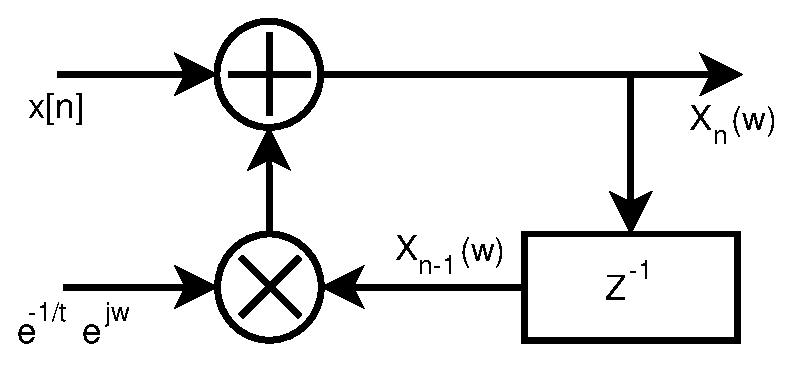
\includegraphics[width=0.75\columnwidth]{Figures/fig_SWIFT_algorithm.eps}
\caption{Structure of a SWIFT algorithm unit to compute the energy in a single frequency bin}
\label{fig:SWIFT_structure}
\end{figure}

It may be noted that while the Windowed Sliding Window DFT is a Discrete Fourier Transform, the SWIFT is continuous in the frequency domain. With $N$ samples in the window, an SDFT will have a normalized frequency resolution of $2\pi/N$. To achieve a finer resolution, an SDFT implementation would have to increase the value of $N$, i.e. the number of samples in the sliding window. This in turn requires additional storage and also reduces the temporal resolution of the DFT. 
In a SWIFT implementation however, a finer frequency resolution doesn't require one to include more samples in the computation. This is an important characteristic of the SWIFT because, for applications where only a subset of the complete frequency spectrum is of interest, it is advantageous to have an algorithm that can increase the frequency resolution without having to increase the digital sample storage. 